\chapter{Algebra Relazionale}
\section{Dai modelli ai linguaggi}
I modelli concettuali e logici permettono di descrivere informazioni, ma non sono direttamente interpretabili da un elaboratore. Dai modelli dobbiamo passare ai linguaggi, dotati di: 
\begin{description}
    \item[sintassi], che definisce le frasi corrette del linguaggio 
    \item[semantica], che definisce le operazioni effettuate quando vengono eseguite gli operatori (o istruzioni o comandi) del linguaggio
\end{description}

\subsection{Linguaggi per Basi di Dati}
\begin{center}
    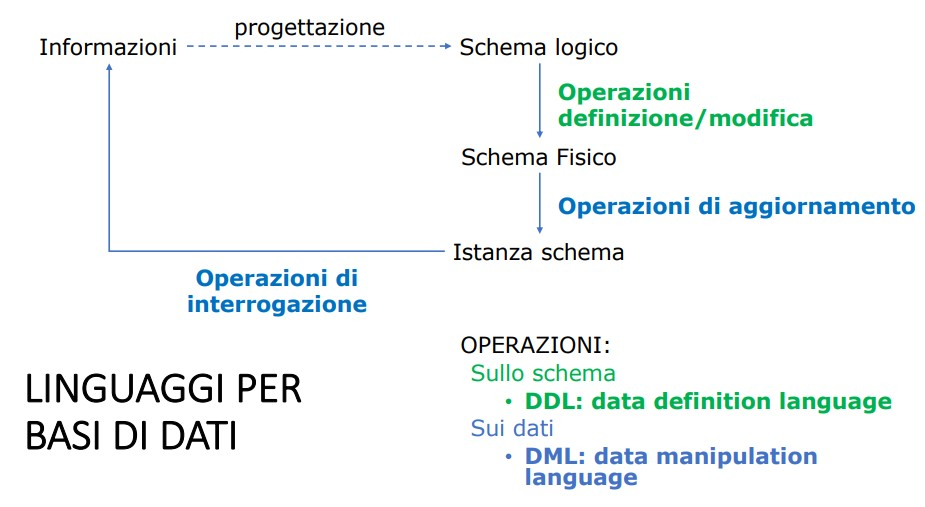
\includegraphics[width=0.675\textwidth]{chaptersLezioniSara/img/AR_linguaggi1.jpg}
\end{center}

\subsection{Tipi di linguaggi}
\subsubsection{Procedurali}
Specificano le modalità di generazione del risultato ("come").
\subsubsection{Dichiarativi}
Specificano le proprietà del risultato ("che cosa").

\subsection{Linguaggi per Basi di Dati Relazionali} 
\begin{description}
    \item[Algebra relazionale]: procedurale
    \item[Calcolo relazionale]: dichiarativo 
    \item[SQL]: (parzialmente) dichiarativo 
    \item[QBE](Query by Example): dichiarativo
\end{description}

\section{AR vs SQL}
Capire l'algebra è la chiave per la comprensione dell'SQL. L'algebra relazionale è un linguaggio procedurale, mentre SQL è un linguaggio dichiarativo.
\begin{center}
    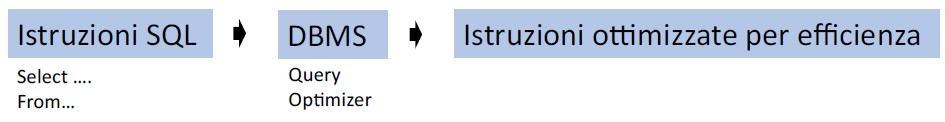
\includegraphics[width=0.675\textwidth]{chaptersLezioniSara/img/AR_linguaggi2.jpg}
\end{center}

\subsubsection{AR}
Linguaggio prettamente formale che forma la base per linguaggi 'reali'.
\\Linguaggio procedurale: si specifica l'algoritmo con cui ottenere il risultato.
\\Istruzioni equivalenti possono differire in termini di efficienza.
\\Relazioni intese in senso matematico => Insiemi di tuple, definite su attributi.
\\Negli insiemi non ci possono essere elementi uguali.

\subsubsection{SQL}
Linguaggio più usato per basi di dati relazionali.
\\Linguaggio (parzialmente) dichiarativo: si specifica il risultato da ottenere senza preoccuparsi di specificare l'algoritmo.
\\Istruzioni equivalenti differiscono solo per leggibilità.
\\Relazioni intese come tabelle.
\\Possono esserci righe uguali.

\section{Algebra Relazionale}
Insieme di operatori:
\begin{itemize}
    \item su relazioni
    \item che producono relazioni
    \item e possono essere composti tra loro a formare nuove interrogazioni
\end{itemize}
\subsubsection{Operatori AR}
\begin{center}
    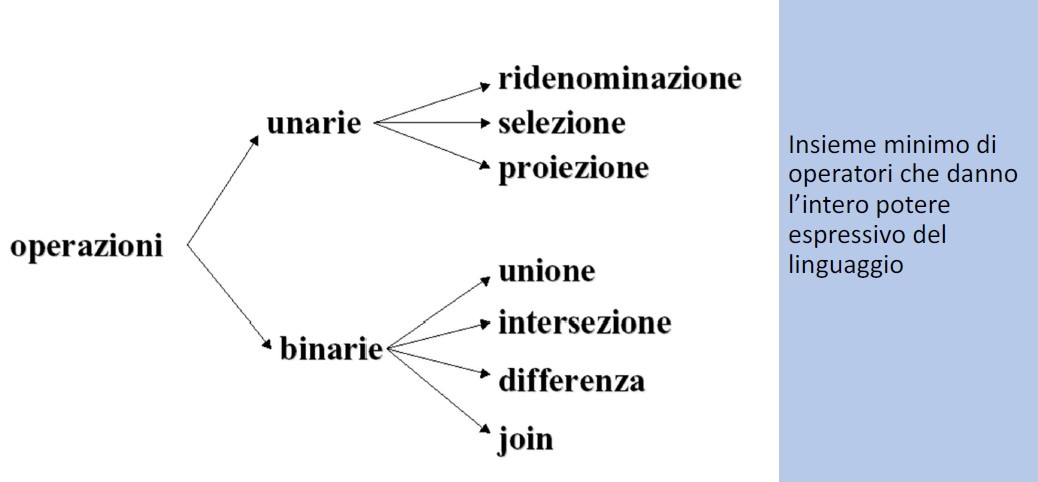
\includegraphics[width=0.675\textwidth]{chaptersLezioniSara/img/AR_operatori1}
\end{center}
\subsubsection{Operatori che vedremo in questa lezione}
\begin{center}
    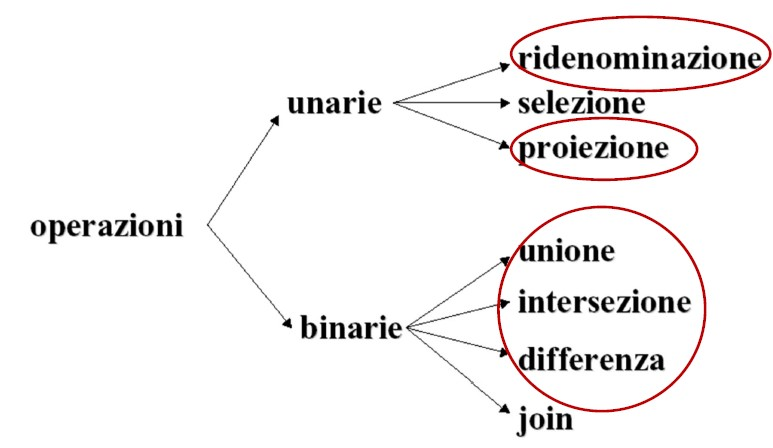
\includegraphics[width=0.675\textwidth]{chaptersLezioniSara/img/AR_operatori2}
\end{center}

\section{Operatori insiemistici}
\subsection{Le relazioni sono insiemi}
In matematica una relazione è un sottoinsieme del prodotto cartesiano di due o più insiemi.
\\Il prodotto cartesiano degli insiemi $D_1, D_2, \dots D_N$ indicato come $D_1 \times D_2 \times \dots \times D_n$ è l'insieme di tutte le n-uple ordinate $(d_1,d_2,\dots,d_n)$ tali che $d_1 \in D_1, d_2 \in D_2, \dots , d_n \in D_n$
% 5 slides di immagini
Una relazione è un insieme quindi:
\begin{itemize}
    \item non c'è ordinamento tra le diverse tuple
    \item le tuple sono distinte (non ce ne possono essere due uguali)
    \item ciascuna tupla è al suo interno ordinata: l'i-esimo valore proviene dall'i-esimo dominio
\end{itemize}
NB: una tabella è una relazione SOLO se non ci sono righe uguali.
\subsection{L'operatore Intersezione}
\subsection{L'operatore Differenza}

\section{Limiti degli operatori insiemistici}
\subsection{L'operatore di ridenominazione}





% www.wooclap.com/SCSYHF